\documentclass[11 pt]{article}
\usepackage{graphics}
\begin{document}
\title{Report- lab $0$}
\author{180020027,180020026,180010021}
\maketitle
\section{Strategy:}
We took greedy approach to solve this problem. The optimal step should be to move forward i.e. to move to three cells in front of you whenever possible, otherwise don't move. The condition to move is as given in the problem i.e. when sensors of current cell and adjacent cell are off.
\section{Result:}
The figure below shows time "Infiltrator" to cross 
the with respect to probability of appearance of head.
\begin{figure}[ht]
\centering 
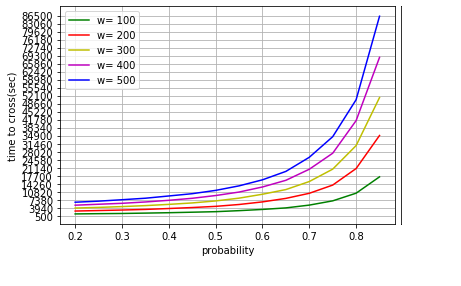
\includegraphics{finalimage.png}
\caption{{\large p v\\s time to cross}}
\label{fig1}
\end{figure}
As one can observe for a given width of border($w$) time to cross border increases non-linearly with increasing slope.
Also at a given $p$ space between adjacent curves seems to be nearly same.

Mathematically,$$ t \propto \frac{w}{(1-p)^2}$$
because we need "sensors" of two cells off at the same time to move one step down. And this is true for all downward steps i.e. w+1 steps to cross the border.

Therefore, mathematical calculations also support what is evident in graph.
\end{document}
